\documentclass[tikz,border=10pt]{standalone}
\usetikzlibrary{positioning, arrows.meta, calc, shapes.geometric, babel}
\usepackage[utf8]{inputenc}
\usepackage[T1]{fontenc}
\usepackage{lmodern}
\usepackage[english]{babel}
\usepackage{amsmath, amssymb, bm}

\begin{document}
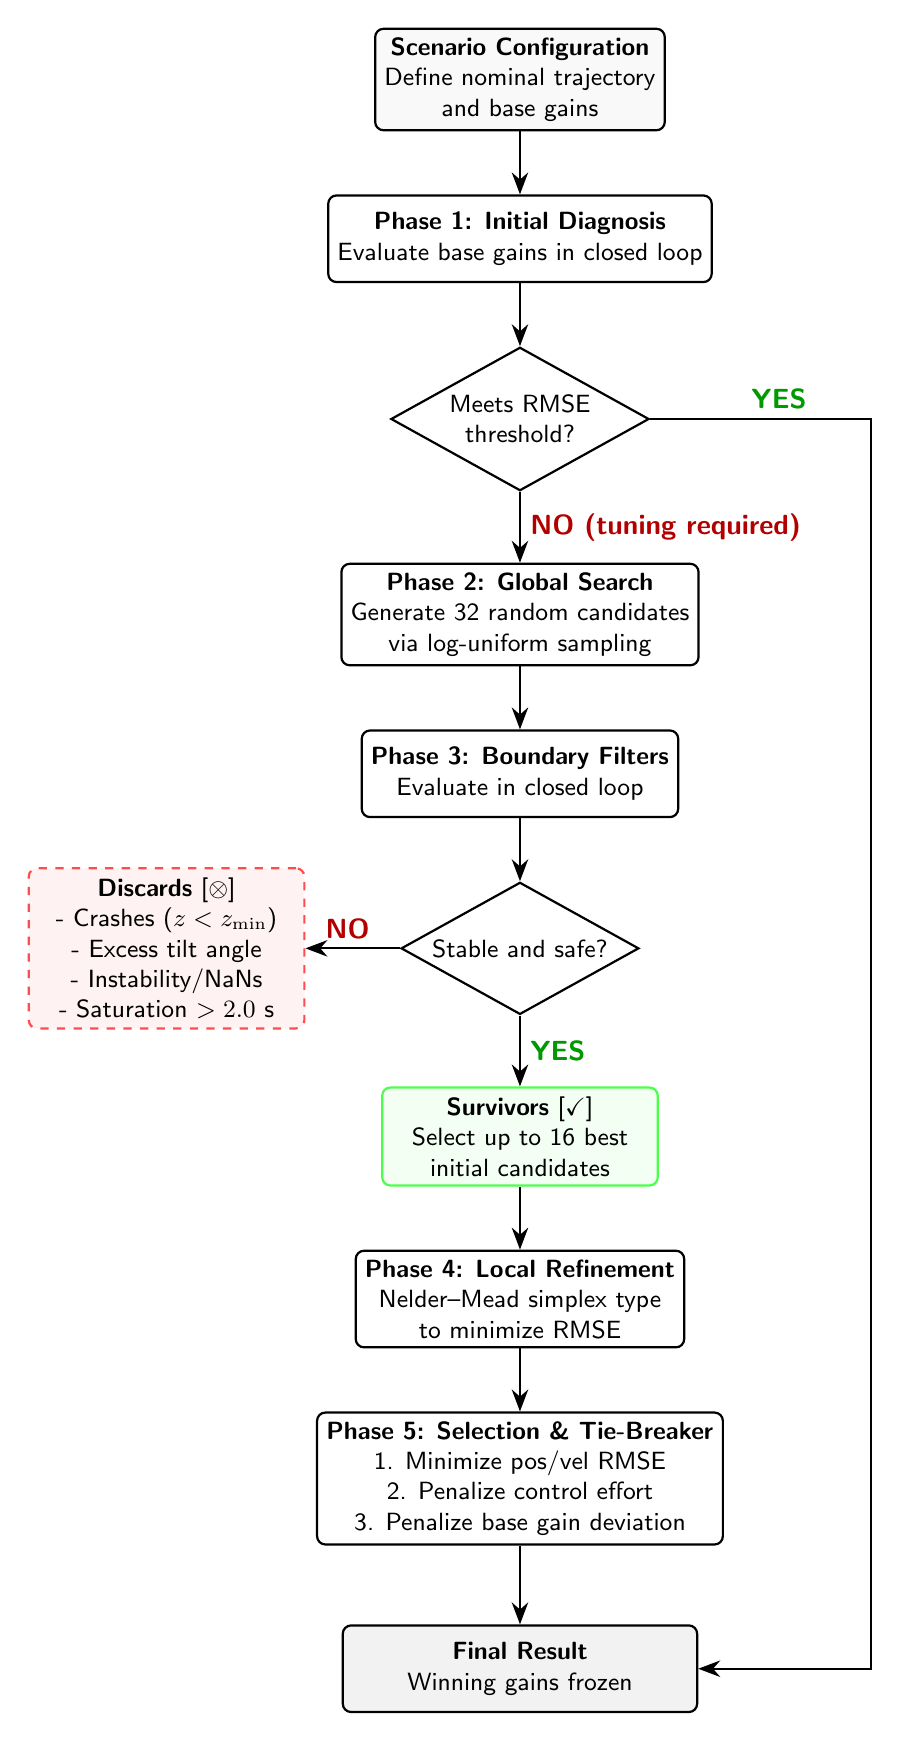
\begin{tikzpicture}[
  node distance=0.8cm and 1.0cm,
  align=center,
  font=\sffamily\small,
  % Estilos de bloques
  box/.style={draw, rectangle, rounded corners=3pt, minimum width=3.5cm, minimum height=1.1cm, thick, fill=white},
  decision/.style={draw, diamond, aspect=1.8, thick, fill=white, inner sep=2pt},
  discardbox/.style={box, fill=red!5, draw=red!70, dashed},
  successbox/.style={box, fill=green!5, draw=green!70},
  % Estilos de flechas
  line/.style={draw, -{Stealth[scale=1.2]}, thick},
  dashline/.style={draw, -{Stealth[scale=1.2]}, thick, dashed}
]

  % ==========================================
  % INITIAL BLOCK: CONFIGURATION
  % ==========================================
  \node[box, fill=gray!5] (inicio) {\textbf{Scenario Configuration}\\Define nominal trajectory\\and base gains};

  % ==========================================
  % PHASE 1: DIAGNOSIS
  % ==========================================
  \node[box, below=of inicio] (diagnostico) {
    \textbf{Phase 1: Initial Diagnosis}\\
    Evaluate base gains in closed loop
  };
  \draw[line] (inicio) -- (diagnostico);

  \node[decision, below=0.8cm of diagnostico] (dec_base) {Meets RMSE\\threshold?};
  \draw[line] (diagnostico) -- (dec_base);

  % ==========================================
  % PHASE 2: GLOBAL SEARCH
  % ==========================================
  \node[box, below=0.9cm of dec_base] (global) {
    \textbf{Phase 2: Global Search}\\
    Generate 32 random candidates\\
    via log-uniform sampling
  };
  % Conexión si NO supera el umbral (requiere sintonización)
  \draw[line] (dec_base) -- node[right, font=\sffamily\bfseries\color{red!70!black}] {NO (tuning required)} (global);

  % ==========================================
  % PHASE 3: BOUNDARY FILTERS
  % ==========================================
  \node[box, below=of global] (filtros) {
    \textbf{Phase 3: Boundary Filters}\\
    Evaluate in closed loop
  };
  \draw[line] (global) -- (filtros);

  % Criterios de filtro
  \node[decision, below=0.8cm of filtros] (dec_filtros) {Stable and safe?};
  \draw[line] (filtros) -- (dec_filtros);

  % Descartes y Aceptación
  \node[discardbox, left=1.2cm of dec_filtros] (descarte) {
    \textbf{Discards} [$\otimes$]\\
    - Crashes ($z < z_{\min}$)\\
    - Excess tilt angle\\
    - Instability/NaNs\\
    - Saturation $> 2.0$ s
  };
  \draw[line] (dec_filtros.west) -- node[above, font=\sffamily\bfseries\color{red!70!black}] {NO} (descarte.east);

  \node[successbox, below=0.9cm of dec_filtros] (supervivientes) {
    \textbf{Survivors} [$\checkmark$]\\
    Select up to 16 best\\
    initial candidates
  };
  \draw[line] (dec_filtros) -- node[right, font=\sffamily\bfseries\color{green!60!black}] {YES} (supervivientes);

  % ==========================================
  % PHASE 4: LOCAL REFINEMENT
  % ==========================================
  \node[box, below=of  supervivientes] (local) {
    \textbf{Phase 4: Local Refinement}\\
    Nelder--Mead simplex type\\
    to minimize RMSE
  };
  \draw[line] (supervivientes) -- (local);

  % ==========================================
  % PHASE 5: MULTI-CRITERIA SELECTION
  % ==========================================
  \node[box, below=of local] (seleccion) {
    \textbf{Phase 5: Selection \& Tie-Breaker}\\
    1. Minimize pos/vel RMSE\\
    2. Penalize control effort\\
    3. Penalize base gain deviation
  };
  \draw[line] (local) -- (seleccion);

  % ==========================================
  % FINAL RESULT: FROZEN YAML
  % ==========================================
  \node[box, fill=gray!10, below=1.0cm of  seleccion, minimum width=4.5cm] (yaml) {
    \textbf{Final Result}\\
    Winning gains frozen
  };
  \draw[line] (seleccion) -- (yaml);

  % Conexión directa desde Fase 1 (SÍ supera el umbral)
  \draw[line] (dec_base.east) -- node[above, xshift=0.3cm, font=\sffamily\bfseries\color{green!60!black}] {YES} ++(2.8,0) |- (yaml.east);

\end{tikzpicture}
\end{document}
